\chapter{Гэрийн даалгаварууд}
\section{Гэрийн даалгавар 1 }
\begin{enumerate}
  \item Үнэний хүснэгтээр шалга: $(P\land Q)\Rightarrow P$.
  \item Үнэний хүснэгтээр шалга: $(P\lor Q)\Leftrightarrow(\lnot P\Rightarrow Q)$.
  \item Эсрэг жишээ ол: "Бүх бүхэл тоо анхны эсвэл тэгш тоо".
  \item Шууд батал: хэрэв $n$ сондгой бол $n^2$ сондгой.
  \item Эсрэгээс нь батал: хэрэв $ab$ сондгой бол $a$ ба $b$ сондгой.
  \item Эквивалент: $(P\Rightarrow Q)\Leftrightarrow(\lnot Q\Rightarrow\lnot P)$.
  \item Батал: $n\equiv0\pmod{5} \Rightarrow n^2\equiv0\pmod{25}$.
  \item Эсрэг жишээ: "Бүх тэгш тоо анхны тоо".
  \item Шууд батал: хэрэв $a,b$ тэгш бол $a+b$ тэгш.
  \item Шууд батал: хэрэв $a$ тэгш бол $a^2+a$ тэгш.
  \item Эсрэгээс нь батал: хэрэв $n^2$ сондгой бол $n$ сондгой.
  \item Эсрэг жишээ: "Хэрэв $ab$ тэгш бол $a$ ба $b$ хоёулаа тэгш".
  \item Батал: $n\equiv0\pmod{3} \Rightarrow n^2\equiv0\pmod{3}$.
  \item Батал: $n\equiv0\pmod{3} \Rightarrow n^3 \equiv 0 \pmod{27}$.
  \item Батал: хэрэв $a$ 4-т хуваагддаг бол $a^2$ 8-д хуваагдана.
  \item Эсрэг жишээ гарга: "Бүх анхны тоо сондгой".
  \item Тавтологи болохыг батал: $((P\Rightarrow Q)\land(Q\Rightarrow R))\Rightarrow(P\Rightarrow R)$.
  \item Тавтологи болохыг батал (resolution): $\big((P\lor Q)\land(\lnot P\lor R)\land(\lnot Q\lor R)\big)\Rightarrow R$.
  \item Дараах өгүүлбэрийн үгүйсгэлийг кванторыг зөв байршуулж бүрэн бич:
        $\forall\,\epsilon>0\,\exists\,\delta>0\,\forall x\,\big(|x-1|<\delta \Rightarrow |f(x)-f(1)|<\epsilon\big)$.
  \item Бүх анхны $p$-ийн хувьд, хэрэв $p\mid n^2$ бол $p\mid n$ болохыг батал.
        (Заавар: Евклидийн лемма $p\mid ab \Rightarrow p\mid a$ эсвэл $p\mid b$.)
  \item $\sqrt{2}+\sqrt{3}$ иррационал болохыг батал.
        (Заавар: эсрэгээс нь $\sqrt{2}+\sqrt{3}=\tfrac{a}{b}$ гэж үзээд квадратлан, $\sqrt{6}$-ыг ашигла.)
  \item Анхны тоо \emph{хязгааргүй олон} байдгийг батал (Евклидийн баталгаа).
  \item (Хүчтэй индукц) Бүх $n\ge 2$-д $n$-ийг анхны тоонуудын үржвэр байдлаар бичиж болохыг батал.
  \item $4k+3$ хэлбэрийн анхны тоо хязгааргүй олон байдаг.
        (Заавар: эсрэгээс нь $p_1,\dots,p_m$ гэж аваад $N=4(p_1\cdots p_m)-1$-ийг авч үз.)
\end{enumerate}
\newpage
\section*{Гэрийн даалгавар 2 }
\begin{enumerate}
  \item Батал: $(A\cup B)\setminus C=(A\setminus C)\cup(B\setminus C)$.
  \item Батал: $(A\cap B)^c=A^c\cup B^c$.
  \item $A\subset \N$ ба дараах нөхцлүүдийг хангах бол $2, 17, 2025, 1000000\in A$ байх уу?
  \begin{enumerate}
      \item $1\in A$
      \item $n\in A\Leftarrow 2n+1\in A$
      \item $3n+1\in A\Leftarrow n\in A$
  \end{enumerate}
  \item $|A|=5$, $|B|=4$, $|A\cap B|=2$. $|A\cup B|$ хэд вэ?
  \item $A\subseteq U$. Батал: $A\cup A^c=U$, $A\cap A^c=\emptyset$.
  \item $A\triangle B=(A\setminus B)\cup(B\setminus A)$. Батал: $A\triangle B=(A\cup B)\setminus(A\cap B)$.
  \item $X=\{0,1\}^3$. $|X|$-ийг ол; элементүүдийг жагсаа.
  \item $f:\mathbb{R}\to\mathbb{R}$, $f(x)=ax+b$. Иньектив/сурьектив байх $a,b$-ийн нөхцөлийг ол.
  \item $f:\mathbb{R}\to\mathbb{R}$, $f(x)=x^2$. Яагаад урвуу үгүй вэ? Ямар домэйнд хязгаарлавал урвуу үүсэх вэ?
  \item $f,g:\mathbb{R}\to\mathbb{R}$ тэгш байвал $f\cdot g$ тэгш болохыг батал.
  \item $f$ сондгой, $g$ сондгой бол $f\cdot g$ тэгш болохыг батал.
  \item $f$ тэгш, $g$ сондгой бол $f\circ g$ сондгой болох эсэхийг шалга.
  \item $h(x)=x^4-3x^2+2$. Тэгш/сондгой эсэхийг дүгнэ.
  \item $p(x)=x^5-2x^3+x$. Тэгш/сондгой эсэхийг дүгнэ.
  \item $a_1=2$, $a_{n+1}=2a_n+1$. Ерөнхий гишүүнийг ол.
  \item $b_1=1$, $b_{n+1}=3b_n-2$. $b_n$-ийг ол.
  \item $g(x)=\dfrac{f(x)-f(-x)}{2}$ бол $g(x)$ сондгой функц байхыг батал.
  \item $d_n=n^2$. Өсөх, үл буурах, буурах аль нь вэ?
  \item $e_n=(-1)^n$. Монотон эсэх? Зааглагдсан эсэх?
  \item $a_n=\dfrac{n}{n+1}$. Монотон эсэх? Дээд/доод хязгаар?
\end{enumerate}
\newpage
\section{Гэрийн даалгавар 3}
\begin{enumerate}
  \item $a+S(b)=S(a+b)$-г $b$-ээр индукцлэн батла.
  \item $S(a)+b=S(a+b)$-г $b$-ээр индукцлэн батла.
  \item $(a+b)^2=a^2+2ab+b^2$ томьёог зөвхөн дистрибутив, коммутатив, ассоциатив чанар ашиглан гарга.
  \item $a\le b\Rightarrow a\cdot c\le b\cdot c$ батал.
  \item $a\le b\Rightarrow a\le b+ c$ батал.
  \item $a\le b$ ба $b<c$ бол $a<c$ батал..
  \item $a\ne 1\Rightarrow \exists!\,m\, a=S(m)$ батал.
  \item $a\cdot b=1\Rightarrow a=1$ ба $b=1$ батал.
  \item $a\le b\iff \exists k,\, b=a+k$ трихотомийг тодорхойлолт ашиглан бүрэн батал.
\end{enumerate}
\newpage
\section{Гэрийн даалгавар 4}
\begin{enumerate}
     \item Реккурент томъёогоор өгөгдсөн дарааллын хувьд:
  \[
    a_1 = 1,\quad a_2 = 1,\quad a_n = a_{n-1} + a_{n-2} \quad (n \geq 3).
  \]
  \begin{enumerate}
    \item $a_6$–г ол.
    \item \[
a_n = \frac{1}{\sqrt{5}} \left( \left( \frac{1+\sqrt{5}}{2} \right)^n - \left( \frac{1-\sqrt{5}}{2} \right)^n \right)
\] индукцээр батал.
\end{enumerate}
\item $(2x - 1)^4$–ийг задла.
\item $x^3 - 3x^2 + 7x - 3$–ийг $x-1$ зэргүүдээр илэрхийлэн бич.
\item $x^3 + x^2 - ax + a-2=0$ тэгшитгэл яг 2 ялгаатай шийдтэй байх бүх $a$ ол.
\item Дараах томьёог батал:
\[
\sin 3x = 3 \sin x - 4 \sin^3 x
\]
\item $\sin \frac{\pi}{6}, \cos \frac{\pi}{3}, \tan \frac{\pi}{4}$ зэрэг утгуудыг өөрөө гарган бич.
\item Дараах томьёог батал: \[
\cos 3x = 4 \cos^3 x - 3 \cos x
\]
\item \(\sin x + \sin y\)-г үржвэрийн хэлбэрт хувиргах томьёог гарга. 
\[
x = \frac{a+b}{2}, \quad y = \frac{a-b}{2}
\]
гэж орлуулснаар \(\sin x + \sin y\)-г \(a, b\)-ийн хувьд бич.
\item $\sin 54^{\circ}$ ол.
\end{enumerate}
\newpage
\section{Семинар ба гэрийн даалгавар 5}
\begin{enumerate}
\item Тригонометрийн урвуу функцтэй холбоотой бодлого
\begin{enumerate}
\item $\arcsin(\frac{1}{2})$–ийн утгыг ол.
\item $\arccos(\frac{1}{2})$–ийн утгыг ол.
\item $\arctan(1)$–ийн утгыг ол.
\item $\arcsin x + \arccos x = \frac{\pi}{2}$–г батал.
\end{enumerate}
\item  Илтгэгч ба логарифм функцтэй холбоотой бодлого
\begin{enumerate}
\item $\ln(e^x) = x$–г батал.
\item $e^{\ln x} = x$–г батал.
\item $\ln(\sqrt{x}) = \frac{1}{2}\ln x$–г батал.
\end{enumerate}
\item Давхар функцтэй холбоотой бодлого
Дараах функцүүдийг $f = g \circ h$ хэлбэрээр бич.
\begin{enumerate}
\item $f(x) = |x^2 - 1|$ 
\item $f(x) = \sqrt{1 - x^2}$ 
\item $f(x) = e^{-x^2}$
\item $f(x) = \cos(2x)$ 
\item $f(x) = (3x - 1)^4$
\item $f(x) = \ln(x^2 + 1)$ 
\item $f(x) = \tan^{-1}(2x)$ 
\item $f(x) = \sqrt{\sin x}$
\end{enumerate}
\item Дараах функцүүдийг $f = g \circ h\circ s$ хэлбэрээр бич.
\begin{enumerate}
\item $f(x) = \frac{1}{\sqrt{1 - x^2}}$
\item $f(x) = \frac{1}{1 + e^{-x}}$ 
\end{enumerate}
\item $f(x) = \dfrac{x^2 - 1}{x + 1}$ функцийн графикийг зур
\item $g(x) = \log_2(x - 3)$ функцийн тодорхойлогдох мужийг ол
\item $h(x) = \arccos(x)$ функцийн утгийн мужийг бич
\item $s(x) = \sin x - \cos x$ функцийг $a\sin (x+\varphi)$ хэлбэрт бичиж утгийн муж ол.
\item Дараах функцийн тодорхойлогдох мужийг ол.
\begin{enumerate}
  \item $y = \log_{x+1}(x^2 - 3x + 2)$ 
  \item $y = \log_6\log_{0.5}(4-x)$ 
  \item $y = \sqrt{5x^2-3x+23}+\lg(x^2 - 10x +16)+\frac{1}{x}$
  \item $y = \sqrt{\log_{0.5}\log_{3}\frac{x+1}{x-1}}$ 
  \item $y = \sqrt{(x^2-3x-10)}\lg\mid x-3\mid $ 
  \item $y = \sqrt{\log_{5-x}(x^2 -9)}$ 
  \item $y = \arccos\!\left(\dfrac{\mid x-1\mid }{x-1} + \dfrac{\mid x-2\mid }{x-2} + \dfrac{\mid x-3\mid }{x-3}\right)$
  \item $y = \arcsin\!\left(\dfrac{\tfrac{x}{3} - \tfrac{3}{x}}{2}\right)$
  \item $y = \lg(\arcsin(\lg x))$
  \item $f(x) = \sqrt{\arcsin x - \arccos x}$
  \item $f(x) = \sqrt{\arccos\!\left(\dfrac{3x+1}{5}\right) - \arcsin\!\left(\dfrac{x+2}{5}\right)}$
  \item $f(x) = \sqrt{\dfrac{5\pi}{6} - \arcsin(2x) - \arccos(6x-2)}$
  \item $f(x) = \sqrt{\dfrac{3\pi}{4} - \arccos x - \arccos(x\sqrt{2}) - \arccos(x\sqrt{3})}$
  \item $f(x) = \sqrt{\sin(\cos x)}$
  \item $f(x) = \sqrt{\sin(\sqrt{x})}$
  \item $f(x) = \sqrt{\tan^2 x - (\sqrt{3}+1)\tan x + \sqrt{3}}$
\end{enumerate}
\item Дараах функцүүдийн утгийн муж ол.
\begin{enumerate}
    \item $f(x) = \sqrt{\dfrac{\sin 3x \cos\!\left(2x - \tfrac{\pi}{6}\right)}{\sin 2x}}$
  \item $f(x) = \sqrt{\cos 3x + \sin x \sin 2x}$
  \item $f(x) = \sqrt{\sin 5x - \cos 3x}$
  \item $f(x) = \sqrt{\dfrac{\cos 3x}{\sin 3x - 2\sin x}} - \tan x$
  \item $f(x) = \cos^2 x + \cos x + 3$
  \item $f(x) = \sin^2 x - 4\sin x + 3$
  \item $f(x) = \sqrt{8 - 2x - x^2}$
  \item $f(x) = \sqrt{2x - 1 - x^2}$
  \item $f(x) = 2^{x^2+4x+5}$
  \item $f(x) = \log_{3}(5 + 4x - x^2)$
  \item $f(x) = \sqrt{2 \log x - (\log x)^2}$
  \item $f'(x) = \sin x - 5\cos x$
  \item $f(x) = \dfrac{\sin x - \cos x}{\sin x + \cos x}$
  \item $f(x) = \log_{2}(\cos x + \sin^2 x)$
  \item $f(x) = 1 - \sqrt{9 - \sqrt{2x^2 + 6\sqrt{2x} + 9}}$
  \item $f(x) =
    \begin{cases}
      2x^2 + 8x + 6, & x < -1, \\
      3\sqrt{x+1}, & x \geq -1
    \end{cases}$
  \item $f(x) =
    \begin{cases}
      \dfrac{8}{x}, & x \leq -2, \\
      x^3 + 4, & -2 < x \leq 0, \\
      \dfrac{4}{x^2 + 1}, & x > 0
    \end{cases}$
  \item $f(x) = \dfrac{x^4 + 6x^3 - 27x - 162}{x^2 + 3x - 18}$
\end{enumerate}
\item Урвуу функц ол.
\begin{enumerate}
    \item $y = x|x| + 2x, \quad x \in \mathbb{R}.$
  \item $y = \dfrac{x^2 + 1}{2x}, \quad x \in [1; +\infty).$
  \item $y = \dfrac{x^2 + 1}{2x}, \quad x \in [0; 1].$
  \item $y = x - \sqrt{x^2 - 1}, \quad x \in (-\infty; -1].$
  \item $y = 2^{x^2 - 2x}, \quad x \in (-\infty; 1].$
  \item $y = 1 - e^{\tfrac{1-x}{1+x}}, \quad x \in \mathbb{R} \setminus \{-1\}.$
  \item $y = \dfrac{3^x - 2^x}{3^x + 2^x}, \quad x \in \mathbb{R}.$
  \item $y = \log_{2}\!\left(x + \sqrt{x^2+1}\right), \quad x \in \mathbb{R}.$
  \item $y = \sin x, \quad x \in \left[-\tfrac{3\pi}{2}, -\tfrac{\pi}{2}\right].$
  \item $y = \sin x, \quad x \in \left[\tfrac{\pi}{2}, \tfrac{3\pi}{2}\right].$
  \item $y = \cos x, \quad x \in [-\pi, 0].$
  \item $y = \cos x, \quad x \in [2\pi, 3\pi].$
\end{enumerate}
\item Дараах функцүүдийн график дүрсэл.
\begin{enumerate}
    \item $f(x) =
    \begin{cases}
      1, & x > 0, \\
     0, & x =0, \\
      -1, & x < 0
    \end{cases}$
     \item $f(x) =
    \begin{cases}
      x+1, & x > 0, \\
     x-1, & -1\leq x < 0, \\
      x^2-1, & x < -1
    \end{cases}$
    \item $f(x)=\sqrt{x^2+2x+1}+\sqrt{x^2-4x+4}$
    \item $f(x)=(x-1)(1-x^4)(x+2)^2$
    \item $f(x)=\dfrac{(x-4)(x^2-9)}{x^2-5x+6}$
    \item $f(x)=\sin^4x-\cos^4 x$
\end{enumerate}
\end{enumerate}
\section{Гэрийн даалгавар 6, 7}
\begin{enumerate}
\item Хязгаарыг тодорхойлолтын дагуу шалга.
\begin{multicols}{2}
\begin{enumerate}
\item $\lim\limits_{x\to 2}\sqrt{x}=\sqrt{2}$ 
\item $\lim\limits_{x\to 2}(3x+5)=11$
\item $\lim\limits_{n\to +\infty}\dfrac{n^2+2n+1}{n^2+n+1}=1$
\item $\lim\limits_{n\to \infty}\dfrac{n}{n+1}=1$
\end{enumerate}
\end{multicols}
\item Хязгаарыг бод.
\begin{multicols}{2}
\begin{enumerate}
\item $\lim\limits_{x\to 1}\dfrac{x^2-1}{x-1}$
\item $\lim\limits_{x\to 4}\dfrac{\sqrt{x}-2}{x-4}$
\item $\lim\limits_{x\to \infty}\dfrac{3x^2+2}{5x^2-7}$
\item $\lim\limits_{x\to \infty}\dfrac{\sqrt{x^2+3}}{x}$
\item $\lim\limits_{x\to 0^+}\dfrac{1}{x}$
\item $\lim\limits _{x\to 1} \dfrac{x^{n+1}-(n+1)x+n}{(x-1)^2}$ 
\item $\lim\limits _{x\to 1} \dfrac{m}{1-x^m}-\dfrac{n}{1-x^n}$
\item $\lim\limits _{x\to +\infty} \dfrac{\sqrt{x+\sqrt{x+\sqrt{x}}}}{\sqrt{x+1}}$
\item $\lim\limits _{x\to +\infty} \dfrac{\sqrt{x}+\sqrt[3]{x}+\sqrt[4]{x}}{\sqrt{2x+1}}$ 
\item $\lim\limits _{x\to 4} \dfrac{\sqrt{1+2x}-3}{\sqrt{x}-2}$
\item $\lim\limits _{x\to 8} \dfrac{\sqrt{1+x}-3}{\sqrt[3]{x}-2}$
\item $\lim\limits_{x\to \infty}\dfrac{2x+3}{5x-1}$
\item $\lim\limits_{x\to -\infty}\dfrac{x^2+1}{2x^2-3}$
\item $\lim\limits_{x\to \infty}\dfrac{2x^3-1}{x^3+5}$
\item $\lim\limits_{x\to 0}\dfrac{\sqrt{1+x}-1}{x}$
\item $\lim\limits_{x\to 0}\dfrac{\ln(1+2x)}{x}$
\item $\lim\limits_{x\to \infty}\dfrac{\sqrt{x^2+5x}}{x}$
\end{enumerate}
\end{multicols}
\item I гайхамшигт хязгаар хэрэглэн хязгаарыг бод.
\begin{multicols}{2}
\begin{enumerate}
\item $\lim\limits_{x\to 0}\dfrac{\sin x}{x}$
\item $\lim\limits_{x\to 0}\dfrac{1-\cos x}{x^2}$
\item $\lim\limits_{x\to 0}\dfrac{\tan x}{x}$
\item $\lim\limits_{x\to 0}\dfrac{\sin(2x)}{x}$
\item $\lim\limits_{x\to 0}\dfrac{\arctan x}{x}$
\item $\lim\limits_{x\to 0}\dfrac{1-\cos(3x)}{x^2}$
\item $\lim\limits_{x\to 0}\dfrac{\sin x - x}{x^3}$
\item $\lim\limits_{n\to \infty}\dfrac{\sin x}{x}$
\item $\lim\limits_{x\to 0}\dfrac{\tan(5x)}{x}$
\item $\lim\limits_{x\to 0}\dfrac{\arcsin x}{x}$
\item $\lim\limits_{x\to 0}\dfrac{\sin x}{1-\cos x}$
\item $\lim\limits_{x\to \frac{\pi}{6}}\dfrac{2\sin x-1}{1-2\cos 2x}$
\end{enumerate}
\end{multicols}
\item  Дараалалын хязгаар бод.
\begin{multicols}{2}
\begin{enumerate}
\item $\lim\limits_{n\to \infty}\dfrac{1}{n}$
\item $\lim\limits_{n\to \infty}\dfrac{2^n}{3^n}$
\item $\lim\limits_{n\to \infty}\dfrac{n!}{n^n}$
\item $\lim\limits_{n\to -\infty}(1+\dfrac{1}{n})^n$
\item $\lim\limits_{n\to \infty}\sqrt[n]{2}$
\item $\lim\limits_{x\to \infty}\sqrt[n]{n}$
\item $\lim\limits_{n\to \infty}\dfrac{n}{2^n}$
\item $\lim\limits_{n\to \infty}\dfrac{2^n}{n!}$
\item $\lim\limits_{n\to \infty}\sqrt[n]{n^2+3}$
\item $\lim\limits_{n\to \infty}\left(1+\dfrac{2}{n}\right)^n$
\item $\lim\limits_{n\to \infty}\dfrac{1}{\sqrt{n}}$
\item $\lim\limits_{n\to \infty}\dfrac{\ln n}{n}$
\item $\lim\limits_{n\to \infty}\dfrac{n}{\ln n}$
\item $\lim\limits_{n\to \infty}\sqrt[n]{3^n+5}$
\item $\lim\limits_{n\to \infty}\dfrac{\sin(1/n)}{1/n}$
\item $\lim\limits_{n\to \infty}(1+\dfrac{1}{n})^{2n}$
\item $\lim\limits_{n\to \infty}\dfrac{(n+1)!}{(n!)^2}$
\item $\lim\limits_{n\to \infty}\dfrac{n^k}{e^n}$ ($k$ тогтмол)
\item $\lim\limits_{n\to \infty}\dfrac{e^n}{n^k}$ ($k$ тогтмол)
\item $\lim\limits_{n\to \infty}\sqrt[n]{n!}$
\item $\lim\limits_{n\to \infty}\dfrac{1+2+\cdots+n}{n^2}$
\item $\lim\limits_{n\to \infty}\dfrac{\sin n}{n^2}$
\end{enumerate}
\end{multicols}
\item II гайхамшигт хязгаар хэрэглэн хязгаарыг бод.
\begin{multicols}{2}
\begin{enumerate}
\item $\lim\limits_{x\to \infty}\dfrac{\ln x}{x}$
\item $\lim\limits_{x\to 1}\dfrac{\ln x}{x-1}$
\item $\lim\limits_{x\to 0}\dfrac{e^{2x}-1}{x}$
\item $\lim\limits_{x\to \infty}\left(1+\dfrac{2}{x}\right)^{3x}$
\item $\lim\limits_{x\to \infty}\dfrac{\ln(x^2+1)}{\ln x}$
\item $\lim\limits_{x\to \infty}\dfrac{x^3}{e^x}$
\item $\lim\limits_{x\to 0}\dfrac{e^x-1}{x}$
\item $\lim\limits_{x\to 0}\dfrac{\ln(1+x)}{x}$
\item $\lim\limits_{x\to \infty}\dfrac{e^x}{x^3}$
\item $\lim\limits_{x\to \infty}\dfrac{\ln x}{\sqrt{x}}$
\end{enumerate}
\end{multicols}
\end{enumerate}
\section{Гэрийн даалгавар 8,9}
\begin{multicols}{2}
\begin{enumerate}
  \item $y = (1 + \sqrt[3]{x})^3$
  \item $y = a \tan\!\left(\dfrac{x}{k} + b\right)$
  \item $y = \sqrt{1 + \sqrt{2px}}$
  \item $y = \arctan(x^2 - 3x + 2)$
  \item $y = \lg(x - \cos x)$
  \item $y = 3\cos^2 x - \cos^3 x$
  \item $y = 5\tan\dfrac{x}{5} + \tan\dfrac{\pi}{8}$
  \item $y = \dfrac{1}{\sqrt[3]{x + \sqrt{x}}}$
  \item $y = \sin\dfrac{x}{2}\sin2x$
  \item $y = \sin(e^{\cos x})$
  \item $y = x^5\sqrt[3]{x^6 - 8}$
  \item $y = e^{-x^2}\ln x$
  \item $y = \left(\sqrt{x} + \dfrac{1}{\sqrt{x}}\right)^{10}$
  \item $y = e^{2x+3}\!\left(x^2 - x + \dfrac{1}{2}\right)$
  \item $y = \dfrac{1}{\sqrt{3}}\arctan\dfrac{x\sqrt{3}}{1 - x^2}$
  \item $y = \dfrac{\tan\dfrac{x}{2} + \cot\dfrac{x}{2}}{x}$
  \item $y = \sin^2\dfrac{x}{3}\cot\dfrac{x}{2}$
  \item $y = \dfrac{\sqrt[5]{4x^6 + 2}}{3x^4}$
  \item $y = \ln\!\left(x + \sqrt{a^2 + x^2}\right)$
  \item $y = x \arctan\sqrt{x}$
  \item $y = \sqrt{1 + \tan^2 x + \tan^4 x}$
  \item $y = \cos2x\ln x$
  \item $y = \dfrac{2}{3}\arctan x + \dfrac{1}{3}\arctan\dfrac{x}{1 - x^2}$
  \item $y = \arcsin(n\sin x)$
  \item $y = x\arcsin\sqrt{\sin x}$
  \item $y = \dfrac{1}{18}\sin^6 3x - \dfrac{1}{24}\sin^8 3x$
  \item $y = x - \sqrt{1 - x^2}\arcsin x$
  \item $y = \sqrt{x + \sqrt{x + \sqrt{x}}}$
  \item $y = \sin^2\dfrac{1 - \ln x}{x}$
  \item $y = \log_3(x^2 - \sin x)$
  \item $y = \arctan\sqrt{\dfrac{1 - x}{1 + x}}$
  \item $y = x\arcsin(\ln x)$
  \item $y = \ln\dfrac{x + \sqrt{1 - x^2}}{x}$
  \item $y = \tan\dfrac{1 - e^x}{1 + e^x}$
\item $y = \dfrac{1 + x \arctan x}{\sqrt{1 + x^2}}$
  \item $y = \dfrac{1}{\cos(x - \cos x)}$
  \item $y = e^x \sin x \cos^3 x$
  \item $y = \sqrt[11]{9 + 6\sqrt{x^9}}$
  \item $y = x - \ln\!\left(2e^x + 1 + \sqrt{e^{2x} + 4e^x + 1}\right)$
  \item $y = e^{\arctan\sqrt{1 + \ln(2x + 3)}}$
  \item $y = \dfrac{e^{x^2}}{e^x + e^{-x}}$
  \item $y = \ln\tan\dfrac{x}{2} - \cot x \ln(1 + \sin x) - x$
  \item $y = 2\ln\!\left(2x - 3\sqrt{1 - 4x^2}\right) - 6\arcsin 2x$
  \item $y = \dfrac{3x^2 - 1}{3x^3} + \ln\sqrt{1 + x^2} + \arctan x$
  \item $y = \dfrac{1}{2}(3 - x)\sqrt{1 - 2x - x^2} + 2\arcsin\dfrac{x + 1}{\sqrt{2}}$
  \item $y = \ln\!\big(x\sin x\sqrt{1 - x^2}\big)$
  \item $y = x\sqrt{1 + x^2}\sin x$
  \item $x = \dfrac{\sqrt{x + 2}(3 - x)^4}{(x + 1)^5}$
  \item $y = \left(1 + x e^{\sqrt{x}}\right)^3$
  \item $y = \dfrac{1}{\sqrt{x}}e^{x^2 - \arctan x + \frac{1}{2}\ln(x + 1)}$
  \item $y = \dfrac{\sin x}{4\cos^4 x} + \dfrac{3\sin x}{8\cos^2 x} + \dfrac{3}{8}\ln\dfrac{1 + \tan\dfrac{x}{2}}{1 - \tan\dfrac{x}{2}}$
  \item $y = \dfrac{x e^x \arctan x}{\ln^5 x}$
  \item $y = \dfrac{(1 - x^2)e^{3x - 1}\cos x}{(\arccos x)^3}$
  \item $y = x\sqrt{(x^2 + a^2)^3} + \dfrac{3a^2 x}{2}\sqrt{x^2 + a^2} + \dfrac{3a^4}{2}\ln\!\left(x + \sqrt{x^2 + a^2}\right)$
  \item $y = x(\arcsin x)^2 - 2x + 2\sqrt{1 - x^2}\arcsin x$
  \item $y = \ln\cos\arctan\dfrac{e^x - e^{-x}}{2}$
  \item $y = -\dfrac{1}{m\sqrt{ab}}\arctan\!\left(e^{mx}\sqrt{\dfrac{a}{b}}\right)$
  \item $y = \dfrac{1}{3}\ln\dfrac{x + 1}{\sqrt{x - x + 1}} + \dfrac{1}{\sqrt{3}}\arctan\dfrac{2x - 1}{\sqrt{3}}$
  \item $y = \ln\dfrac{\sqrt{1 + x} - \sqrt{1 - x}}{\sqrt{1 + x} + \sqrt{1 - x}} + 2\arctan\sqrt{\dfrac{1 - x}{1 + x}}$
\end{enumerate}
\end{multicols}
\newpage
\section{Семинар 10}
\begin{enumerate}
    \item Дараах функцүүдийн заагдсан эрэмбийн уламжлалыг ол.
\begin{enumerate}
  \item $y = x^2 - 3x + 2,\quad y'' = ?$
  \item $y=1-x^2-x^4, \quad y'''=?$
  \item $y=(1+x)^6, \quad y'''(2)=?$
  \item $y=(x^3+1)^8, \quad y'''=?$
  \item $y=\cos ^2 x, \quad y'''=?$
  \item $y=\dfrac{1}{1-x}, \quad y^{(5)}=?$
  \item $y = xe^{x^2},\quad y'' = ?$
  \item $y = x^3\ln(x),\quad y^{(4)} = ?$
  \item $y = \ln(x+\sqrt{1+x^2}),\quad y'' = ?$
  \item $y = \sqrt{1-x^2}\arcsin x,\quad y'' = ?$
\end{enumerate}
\item Дараах функцүүдийн $n$ эрэмбийн уламжлалыг ол.
\begin{enumerate}
   
  \item $y = e^{ax}$
  \item $y = e^{-x}$
  \item $y = \sin^2x$
  \item $y = xe^x$
  \item $y = x\ln x$
  \item $y = (x^2+x-1)\cos x$
  \item $y = e^{x}\cos x$
  \item $y = x^{n-1}e^{\frac{1}{x}}$
\end{enumerate}
\item Далд функцийн уламжлал ол.
\begin{enumerate}
    \item $\dfrac{x^2}{a^2}+\dfrac{y^2}{b^2}-1=0$ , $\dfrac{d^2y}{dx^2}$
    \item $y=\tan(x+y)$ , $\dfrac{d^3y}{dx^3}$
    \item $y^3+x^3-3axy=0$ , $y''$
    \item $e^{x+y}-xy=0$ , $y''$
\end{enumerate}
\item Параметр функцийн уламжлал ол.
\begin{enumerate}
    \item
    $\begin{cases}
        x=at^2\\
        y=bt^3
    \end{cases}$ , $\dfrac{d^2y}{dx^2}$
      \item 
     $ \begin{cases}
        x=a\cos t\\
        y=b\sin t
    \end{cases} , \dfrac{d^3y}{dx^3}$
      \item 
      $\begin{cases}
        x=t-\sin t\\
        y=1-\cos t
    \end{cases} , \dfrac{d^2y}{dx^2}$
      \item 
      $\begin{cases}
        x=\ln t\\
        y=t^2-1
    \end{cases} , \dfrac{d^3y}{dx^3}$  
    \item 
    $\begin{cases}
        x=e^t\sin t\\
        y=e^t\cos t
    \end{cases}$ бол $y''(x+y)^2-2(xy'-y)=0$ биелэхийг батал.
\end{enumerate}
\end{enumerate}
\newpage
\section{Гэрийн даалгавар 11}
\begin{enumerate}
  \item Функцийн локал экстремумыг ол.
  \begin{enumerate}
  \item  $y = x^3 - 6x^2 + 9x - 4$ 
  \item $y = 2x^3 - x^4$ 
  \item $y = x(x-1)^3(x-2)^3$ 
  \item $y = x + \dfrac{1}{x}$ 
  \item $y = \dfrac{2x}{1+x^2}$ 
  \item $y = \dfrac{x^3 - 3x + 2}{x^3 + 2x + 1}$ 
  \item $y = \sqrt{2x - x^3}$ 
  \item $y = x^3\sqrt[3]{x - 1}$ 
  \item $y = x e^{-x}$
  \item $y = \sqrt{x}\,\ln x$ 
  \item $y = \dfrac{(\ln x)^2}{x}$
  \item $y = \cos x + \dfrac{1}{2}\cos 2x$ 
  \item $y = \dfrac{10}{1 + \sin^2 x}$ 
  \item $y = \arctan x - \dfrac{1}{2}\ln(1 + x^2)$ 
  \item $y = e^x \sin x$ 
  \item $y = |x|\, e^{-|x-1|}$
  \end{enumerate}
\item Өгөгдсөн завсар дээрх хамгийн их ба хамгийн бага утгыг ол.
  \begin{enumerate}
  \item  $f(x) = 2x$, $[-1; 5]$ 
  \item $f(x) = x^2 - 4x + 6$, $[-3; 10]$ 
  \item $f(x) = |x^2 - 3x + 2|$, $[-10; 10]$ 
  \item $f(x) = x + \dfrac{1}{x}$, $[0.01; 100]$ 
  \item $f(x) = \sqrt{5 - 4x}$, $[-1; 1]$ 
  \end{enumerate}
\item Дараах тэнцэтгэл бишүүдийг функцийн хамгийн их ба бага утга олох замаар батла.
   \begin{enumerate}
   \item $|3x - x^3| \le 2$, хэрэв $|x| \le 2$
   \item $\dfrac{1}{2^{p-1}} \le x^p + (1-x)^p \le 1$, хэрэв $0 \le x \le 1$ ба $p>1$.
  \item $x^m (a-x)^n \le 
    \dfrac{m^m n^n}{(m+n)^{m+n}}\, a^{m+n}$, хэрэв $m>0$, $n>0$, $0\le x\le a$.
  \item $\dfrac{x+a}{2^{(n-1)/n}} \le \sqrt[n]{x^n+a^n} \le x+a$, хэрэв $x>0,\, a>0,\, n>1$.
  \item $|a\sin x + b\cos x| \le \sqrt{a^2+b^2}$.
  \item $\dfrac{2}{3} \le \dfrac{x^2+1}{x^3+x+1} \le 2$, бүх $x \in \mathbb{R}$-д.
   \end{enumerate}
\item $y=ax^2+bx+c$ параболын $x=p, x=q$ цэгүүд дээрх шүргэгч шулуунууд $x=\dfrac{p+q}{2}$ цэг дээр огтолцохыг батал.
\item $y=x^2$ параболын $x=p, x=q$ цэгүүд дээрх шүргэгч шулуунууд перпиндикуляр бол огтолцолын цэг нь $y=-\dfrac{1}{4}$ шулуун дээр оршихыг батал.
\item $y=\dfrac{1}{x}$ функцийн $x=p ,\quad (p>0)$ цэг дээрх шүргэгч шулуун ба $ox$, $oy$ тэнхлэгүүдээр үүсэх гурвалжны талбай $p$-с хамаарахгүй тогтмол байхыг батал.
\end{enumerate}
\newpage
\section{Гэрийн даалгавар 12}
\begin{enumerate}
\begin{multicols}{2}
  \item Лопиталын дүрэм хэрэглэн хязгаар бод.
\begin{enumerate}
 \item $\displaystyle \lim_{x\to 0}  \frac{e^{ax}-\cos(\alpha x)}{e^{\beta x}-\cos(\beta x)}.$
 \item $\displaystyle \lim_{x\to 0} \frac{e^{a\sqrt{x}}-1}{\sqrt{\sin(bx)}}.$
\item $\displaystyle\lim_{x\to \infty} 
     \frac{\pi-2\arctan x}{\ln(1+\tfrac{1}{x})}.$
  \item $\displaystyle \lim_{x\to 0} \frac{\ln(\cos x)}{x}.$
  \item $\displaystyle \lim_{x\to a} \frac{x^{m}-a^{m}}{x^{n}-a^{n}}.$

  \item $\displaystyle\lim_{x\to 0} 
     \frac{a^{x}-b^{x}}{c^{x}-d^{x}}.$

  \item $\displaystyle \lim_{x\to 0} 
     \frac{e^{x}-e^{-x}}{\sin x \cos x}.$
  \item $\displaystyle \lim_{x\to 1} 
     \frac{\ln(1-x)+\tan\frac{\pi x}{2}}{\cot(\pi x)}.$

  \item $\displaystyle \lim_{x\to +\infty} x^{n} e^{-x}.$

  \item $\displaystyle \lim_{x\to \infty} 
     \bigl[(\pi - 2\arctan x)\ln x\bigr].$

  \item $\displaystyle \lim_{x\to \infty} 
     \left[x\sin\frac{a}{x}\right].$

  \item $\displaystyle  \lim_{\varphi \to a} 
     \left[(a^{2}-\varphi^{2}) \tan\frac{\pi\varphi}{2a}\right].$

  \item $\displaystyle \lim_{x\to 1} 
     \left(\frac{1}{\ln x} - \frac{x}{\ln x}\right).$

  \item $\displaystyle  \lim_{x\to 0} 
     \left(\cot x - \frac{1}{x}\right).$

  \item $\displaystyle \lim_{x\to \infty} 
     \frac{1}{\cos\frac{\pi x}{2}\,\ln(1-x)}.$

  \item $\displaystyle \lim_{x\to \infty} 
     \left[\sqrt[n]{(a+x)(b+x)(c+x)} - x\right].$

  \item $\displaystyle  \lim_{x\to 0} 
     \left[x^{2} e^{\frac{1}{x^{2}}}\right].$

  \item $\displaystyle \lim_{x\to \frac{\pi}{2}}
     \left(\tan x\right)^{2x-\pi}.$

  \item $\displaystyle \lim_{x\to 0} 
     x^{\frac{1}{\ln(e^{x}-1)}}.$

  \item $\displaystyle  \lim_{x\to 0} 
     \left(\frac{1}{x}\right)^{\tan x}.$

  \item $\displaystyle  \lim_{x\to \infty} 
     \left(e^{x}+e^{-x}\right)^{1/x}.$

  \item $\displaystyle  \lim_{x\to a} 
     \left(2 - \frac{x}{a}\right)^{\frac{\tan(\pi x / 2a)}{}}.$ 
\end{enumerate}
\item Дараах функцүүдийн локал экстермум, нугаралтын
цэгүүдийг олж, хотгор ба гүдгэр
интервалыг тодорхойл.
\begin{enumerate}
 \item $y = 3x^{5} - 5x^{4} + 3x - 2$;
  \item $y = (x+2)^{6} + 2x + 2$;
  \item $y = -\dfrac{x^{3}}{x^{2} + 3a^{2}},\quad a>0$;
  \item $y = a - \sqrt[3]{x-b}$;
  \item $y = e^{\sin x},\quad -\dfrac{\pi}{2} \le x \le \dfrac{\pi}{2}$;
  \item $y = \dfrac{a}{x}\ln\!\frac{x}{a},\quad a>0$;
  \item $y = a - \sqrt[5]{(x-b)^{2}}$;
  \item $y = e^{\arctan x}$;
  \item $y = x^{4}\bigl(12\ln x - 7\bigr)$;
\item $y = x\sqrt{2-x^2}$

\item $y = \operatorname{ch}(ax)$

\item $y = x^2 e^{-x}$

\item $y = \frac{x}{\ln x}$

\item $y = x^{1/x}$
\end{enumerate}
\item Тэйлорын теорем
\begin{enumerate}
\item $y = \frac{e^x + e^{-x}}{2}$ функцийг $x_0=0$ орчимд Тэйлорын $2n$-р эрэмбийн томьёо бич.

\item $y = x^3 \ln x$ функцийг $x_0 = 1$ орчимд Тэйлорын $n$-р эрэмбийн томьёо бич.

\item $f(x)=x^8-2x^7+5x^6-x+3$.  
$x_0=2$ орчимд Тэйлорын эхний 3 гишүүн олж, $f(2.02)$ ба $f(1.97)$-ыг ойролцоол.

\item $f(x)=x^{80}-x^{40}+x^{20}$.  
$x_0=1$ орчимд $(x-1)$ зэргийн хувьд Тэйлорын эхний 3 гишүүн олж, $f(1.005)$-ыг ойролцоол.
\end{enumerate}
\item Функц зохион хамгийн их бага ута ол.
\begin{enumerate}

\item Үүсгэгч урт $20$ см байх конус хэлбэрийн воронка хийх. Эзэлхүүн хамгийн их байх өндөрийг ол.

\item Төв өнцөг нь $\alpha$ байх дугуйны секторыг эвхэж конус үүсгэвэл, эзэлхүүн хамгийн их байх $\alpha$ өнцгийг ол.

\item Периметр нь $2p$ бодит тэгш өнцөгт гурвалжинг эргүүлэхэд үүсэх биетийн эзэлхүүн хамгийн их байх гурвалжны хэмжээг ол.
\end{enumerate}
\end{multicols}
\end{enumerate}
\section{Гэрийн даалгавар 13}
\begin{enumerate}
\begin{multicols}{2}
  \item $\displaystyle \int \frac{dx}{2x-1}.$
  \item $\displaystyle \int \frac{dx}{cx+m}.$
  \item $\displaystyle \int \frac{x\,dx}{x^{2}+1}.$

  \item $\displaystyle \int \frac{x^{2}\,dx}{x^{3}+1}.$
  \item $\displaystyle \int \frac{e^{x} dx}{e^{x}+1}.$
  \item $\displaystyle \int \frac{e^{2x} dx}{e^{2x}+a^{2}}.$

  \item $\displaystyle \int \tan x\, dx.$
  \item $\displaystyle \int \cot x\, dx.$
  \item $\displaystyle \int \tan 3x\, dx.$

  \item $\displaystyle \int \cot(2x+1)\, dx.$
  \item $\displaystyle \int \frac{\sin 2x}{1+\cos^{2}x}\, dx.$
  \item $\displaystyle \int \frac{dx}{x \ln x}.$

  \item $\displaystyle \int \frac{(\ln x)^{m}}{x}\, dx.$
  \item $\displaystyle \int e^{\sin x}\, d(\sin x).$
  \item $\displaystyle \int e^{\sin x}\cos x\, dx.$

  \item $\displaystyle \int a^{3x}\, dx.$
  \item $\displaystyle \int a^{-x}\, dx.$

  \item $\displaystyle \int e^{-3x+1}\, dx.$
  \item $\displaystyle \int e^{x^{2}} x\, dx.$
  \item $\displaystyle \int e^{-x^{3}} x^{2}\, dx.$

  \item $\displaystyle \int \frac{d\left(\frac{x}{3}\right)}{\sqrt{1-\left(\frac{x}{3}\right)^{2}}}.$
  \item $\displaystyle \int \frac{dx}{\sqrt{1-25x^{2}}}.$
  \item $\displaystyle \int \frac{dx}{1+9x^{2}}.$

  \item $\displaystyle \int \frac{dx}{\sqrt{4-x^{2}}}.$
  \item $\displaystyle \int \frac{dx}{2x^{2}+9}.$
  \item $\displaystyle \int \frac{dx}{\sqrt{4-9x^{2}}}.$

  \item $\displaystyle \int \frac{x\, dx}{x^{4}+1}.$
  \item $\displaystyle \int \frac{x\, dx}{a^{2}-x^{4}}.$
  \item $\displaystyle \int \frac{x^{2} dx}{x^{6}+4}.$

  \item $\displaystyle \int \frac{x^{3} dx}{\sqrt{1-x^{8}}}.$
  \item $\displaystyle \int \frac{e^{x} dx}{e^{2x}+4}.$
  \item $\displaystyle \int \frac{2^{x} dx}{\sqrt{1-4^{x}}}.$

  \item $\displaystyle \int \frac{\cos\alpha\, d\alpha}{a^{2}+\sin^{2}\alpha}.$
  \item $\displaystyle \int \frac{e^{2x}-1}{e^{x}}\, dx.$
  \item $\displaystyle \int (e^{x}+1)^{3} dx.$

  \item $\displaystyle \int \frac{1+x}{\sqrt{1-x^{2}}}\, dx.$
  \item $\displaystyle \int \frac{8x-1}{x^{2}+9} dx.$
  \item $\displaystyle \int \frac{\sqrt{1-x}}{1+x}\, dx.$

  \item $\displaystyle \int \frac{x(1-x^{2})}{1+x^{4}}\, dx.$
  \item $\displaystyle \int \frac{1+x-x^{2}}{\sqrt{(1-x^{2})^{3}}}\, dx.$
  \item$\displaystyle \int \frac{dx}{(x+\sqrt{x^{2}-1})^{2}}.$ 
\end{multicols}
\end{enumerate}
\section{Гэрийн даалгавар 14} Тохиромжтой аргаар бод.
\begin{enumerate}
\begin{multicols}{2}
\item $\displaystyle \int \frac{dx}{x^6(1+x^2)}.$

\item $\displaystyle \int \frac{x^2}{(1-x^2)^3}\,dx.$

\item $\displaystyle \int \frac{dx}{1+x^4+x^8}.$

\item $\displaystyle \int \frac{dx}{\sqrt{x+\sqrt[3]{x}}}.$

% ----------- 51–55 -----------
\item $\displaystyle \int x^2\sqrt{\frac{x}{1-x}}\,dx.$

\item $\displaystyle \int \frac{x+2}{x^2\sqrt{1-x^2}}\,dx.$

\item $\displaystyle \int \sqrt{\frac{x}{1-x}}\,dx.$
\item $\displaystyle \int \frac{dx}{\sqrt[3]{x^2(1-x)}}.$

\item $\displaystyle \int \frac{dx}{x\sqrt{1+x^3+x^6}}.$

% ----------- 11–15 -----------
\item $\displaystyle \int x\sqrt{x^4-2x^2-1}\,dx.$

\item $\displaystyle \int \frac{1+\sqrt{\frac{1-x}{1+x}}}{1-\sqrt{\frac{1-x}{1+x}}}\,dx.$

\item $\displaystyle \int \frac{(1+x)\,dx}{\sqrt{1+x^2}}.$

\item $\displaystyle \int \frac{\ln(1+x+x^2)}{(1+x)^2}\,dx.$

\item $\displaystyle \int (2x+3)\arccos(2x-3)\,dx.$

% ----------- 16–20 -----------
\item $\displaystyle \int x\ln(4+x^4)\,dx.$

\item $\displaystyle \int \frac{\arcsin x}{x^2}\cdot\frac{1+x^2}{\sqrt{1-x^2}}\,dx.$

\item $\displaystyle \int \frac{x\ln\!\left(1+\sqrt{1+x^2}\,\right)}{\sqrt{1+x^2}}\,dx.$

\item $\displaystyle \int x\sqrt{x^2+1}\,\ln\!\sqrt{x^2-1}\,dx.$

\item $\displaystyle \int \frac{x}{\sqrt{1-x^2}}\ln\frac{x}{\sqrt{1-x}}\,dx.$

% ----------- 21–25 -----------
\item $\displaystyle \int \frac{dx}{(2+\sin x)^2}.$

\item $\displaystyle \int \frac{\sin 4x}{\sin^8 x+\cos^8 x}\,dx.$

\item $\displaystyle \int \frac{\sin x}{\sqrt{1+\cos x}}\,dx.$

\item $\displaystyle \int \frac{ax^2+b}{x^2+1}\arctan x\,dx.$

\item $\displaystyle \int \frac{ax^2+b}{x^2-1}\ln\!\left|\frac{x-1}{x+1}\right|dx.$

% ----------- 26–30 -----------
\item $\displaystyle \int \frac{x\ln x}{(1+x^2)^2}\,dx.$

\item $\displaystyle \int \frac{x\arctan x}{\sqrt{1+x^2}}\,dx.$

\item $\displaystyle \int \frac{\sin 2x}{\sqrt{1+\cos^4 x}}\,dx.$

\item $\displaystyle \int \frac{x^3\arccos x}{\sqrt{1-x^2}}\,dx.$

\item $\displaystyle \int \frac{x^4\arctan x}{1+x^2}\,dx.$

% ----------- 31–35 -----------
\item $\displaystyle \int \frac{x\arctan x}{(1+x^2)^3}\,dx.$

\item $\displaystyle \int \frac{x\ln\!\left(x+\sqrt{1+x^2}\right)}{(1-x^2)^2}\,dx.$

\item $\displaystyle \int \sqrt{1-x^2}\,\arcsin x\,dx.$

\item $\displaystyle \int x(1+x^2)\arctan x\,dx.$

\item $\displaystyle \int x^x(1+\ln x)\,dx.$

% ----------- 36–40 -----------
\item $\displaystyle \int \frac{\arcsin(e^x)}{e^x}\,dx.$

\item $\displaystyle \int \frac{\arctan \frac{x}{2}}{e^x(1+e^x)}\,dx.$

\item $\displaystyle \int \frac{dx}{(e^{x+1}+1)^2-(e^{x-1}+1)^2}.$

\item $\displaystyle \int \sqrt{\tanh^2 x+1}\,dx.$

\item $\displaystyle \int \frac{1+\sin x}{1+\cos x}e^x\,dx.$

% ----------- 41–45 -----------
\item $\displaystyle \int |x|\,dx.$

\item $\displaystyle \int x\,|x|\,dx.$

\item $\displaystyle \int (x+|x|)^2\,dx.$

\item $\displaystyle \int (1+|x|-|1-x|)\,dx.$

\item $\displaystyle \int (e^{-1/x})\,dx.$

% ----------- 46–50 -----------
\item $\displaystyle \int \max(1, x^3)\,dx.$

\item $\displaystyle \int \frac{x^5}{\sqrt{1+x^2}}\,dx.$
\item $\displaystyle \int \varphi(x)\,dx$, \quad энд $\varphi(x)$ нь $x$ тооноос ойрхон бүхэл тоо хүртэлх зай.

\item $\displaystyle \int \lfloor x \rfloor\, |\sin \pi x|\, dx \qquad (x>0).$

\item $\displaystyle \int f(x)\,dx$, \quad энд
\[
f(x)=
\begin{cases}
1 - x^2, & |x|\le 1,\\
1 - |x|, & |x|>1.
\end{cases}
\]

\item $\displaystyle \int f(x)\,dx$, \quad энд
\[
f(x)=
\begin{cases}
1, & x<0,\\[4pt]
x+1, & 0\le x \le 1,\\[4pt]
2x, & x>1.
\end{cases}
\]

\item $\displaystyle \int x\, f''(x)\,dx.$

% ----------- 6–10 -----------
\item $\displaystyle \int f'(2x)\,dx.$

\item $f(x)$–ийг ол, хэрэв $\; f'(x^2)=\dfrac1{x}\quad (x>0).$

\item $f(x)$–ийг ол, хэрэв $\; f'(\sin^2 x)=\cos^2 x.$

\end{multicols}
\end{enumerate}
\newpage
\section{Семинар ба Гэрийн даалгавар 15}
\begin{enumerate}
    \item Доорх функцуудын хувьд өгөгдсөн завсрыг 
$n=4$ адил урттай хуваагаад 
\[
\sum_{k=1}^4 f(x_k^*)\,\Delta x
\]
 нийлбэрийг тооцоол.
Энд $x_k^*$ нь дараах гурван тохиолдлоор авна:
\begin{enumerate}
\item[a)]  завсрын \textbf{зүүн} төгсгөл
\item[b)]  завсрын \textbf{дундаж} цэг
\item[c)]  завсрын \textbf{баруун} төгсгөл
\end{enumerate}

Бүх тохиолдолд график зурж, тухайн нийлбэрийг илэрхийлж буй тэгш өнцөгтүүдийн талбайг харуул.
\begin{enumerate}
\item $f(x)=3x+1$, \quad завсар: $[2,\,6]$

\item $f(x)=\frac{1}{x}$, \quad завсар: $[1,\,9]$

\item $f(x)=\cos x$, \quad завсар: $[0,\,\pi]$

\item $f(x)=2x-x^2$, \quad завсар: $[-1,\,3]$
\end{enumerate}
\item \[
f(x)=
\begin{cases}
|x-2|, & x\ge0,\\[4pt]
x+2, & x<0.
\end{cases}
\] бол дараах интегралуудыг ол.
\begin{enumerate}
\begin{multicols}{2}
\item $\displaystyle\int_{-2}^{0} f(x)\,dx$
\item $\displaystyle\int_{-2}^{2} f(x)\,dx$
\item $\displaystyle\int_{0}^{6} f(x)\,dx$
\item $\displaystyle\int_{-4}^{6} f(x)\,dx$  
\end{multicols}
\end{enumerate}
\item 
\[
f(x)=
\begin{cases}
2x, & x\le1,\\[4pt]
2, & x>1.
\end{cases}
\]
бол дараах интегралуудыг ол.
\begin{enumerate}
\begin{multicols}{2}
\item $\displaystyle\int_{0}^{1} f(x)\,dx$
\item $\displaystyle\int_{-1}^{1} f(x)\,dx$
\item $\displaystyle\int_{1}^{10} f(x)\,dx$
\item $\displaystyle\int_{1/2}^{5} f(x)\,dx$
\end{multicols}
\end{enumerate}
\item Доорх зураг нь $y=f(x)$ муруй ба $ox$ тэнхлэгийн хоорондох талбайн утгуудыг өгөв. Тэдгээрийг ашиглан 
$$
\int_a^b f(x)\,dx,\quad
\int_b^c f(x)\,dx,\quad
\int_a^c f(x)\,dx,\quad
\int_a^d f(x)\,dx
$$ интегралуудыг ол.
\begin{figure}[h]
\centering
\begin{tikzpicture}[scale=1.5]
  % axes
  \draw[->] (-0.2,0) -- (5.2,0) node[right]{$x$};
  \draw[->] (0,-1) -- (0,2) node[above]{$y$};

  % points a<b<c<d on x-axis
  \coordinate (A) at (0.5,0);
  \coordinate (B) at (1.5,0);
  \coordinate (C) at (2.8,0);
  \coordinate (D) at (4.5,0);

  \node[below] at (A) {$a$};
  \node[below] at (B) {$b$};
  \node[below] at (C) {$c$};
  \node[below] at (D) {$d$};

  % curve (just a smooth spline)
  \draw[thick,domain=0.3:4.7,smooth]
     plot(\x,{0.8*sin(120*\x)+0.3*\x-0.5});

  % shaded areas: [a,b] positive 0.8
  \fill[blue!20] (A) --
    plot[domain=0.5:1.5,smooth] (\x,{0.8*sin(120*\x)+0.3*\x-0.5}) --
    (B) -- cycle;
  \node at (1,0.6) {\small  талбай$=0.8$};

  % [b,c] negative 2.6
  \fill[cyan!25] (B) --
    plot[domain=1.5:3,smooth] (\x,{0.8*sin(120*\x)+0.3*\x-0.5}) --
    (C) -- cycle;
  \node at (2.2,-1) {\small талбай $=1$};

  % [c,d] positive 1.5
  \fill[red!20] (C) --
    plot[domain=3:4.5,smooth] (\x,{0.8*sin(120*\x)+0.3*\x-0.5}) --
    (D) -- cycle;
  \node at (3.8,1.2) {\small талбай $=1.6$};

  \node[right] at (4.7,1.8) {$y=f(x)$};
\end{tikzpicture}
\end{figure}

\item Дараах функцүүдийн график ба $ox$ тэнхлэгийн өгөгдсөн интервалаар хүрээлэгдсэн хэсгийн талбайг ол.
\begin{enumerate}
\begin{multicols}{2}
\item $f(x)=x^3,\quad [2,3]$
\item $f(x)=x^4,\quad [-1,1]$
\item $f(x)=3\sqrt{x},\quad [1,4]$
\item $f(x)=x^{-2/3},\quad [1,27]$
\item $f(x)=e^{2x},\quad [0,\ln2]$
\item $f(x)=\dfrac1x,\quad [1,5]$
\end{multicols}
\end{enumerate}

\item Дараах интегралуудыг Ньютон-Лейбницийн теоремийг ашиглан бод.

\begin{enumerate}
\begin{multicols}{2}
\item $\displaystyle\int_{-2}^{1}(x^2-6x+12)\,dx$
\item $\displaystyle\int_{-1}^{2}4x(1-x^2)\,dx$
\item $\displaystyle\int_{1}^{4}\frac{4}{x^2}\,dx$
\item $\displaystyle\int_{1}^{2}\frac1{x^6}\,dx$
\item $\displaystyle\int_{4}^{9}2x\sqrt{x}\,dx$
\item $\displaystyle\int_{1}^{4}\frac1{x\sqrt{x}}\,dx$
\item $\displaystyle\int_{-\pi/2}^{\pi/2}\sin\theta\,d\theta$
\item $\displaystyle\int_{0}^{\pi/4}\sec^2\theta\,d\theta$
\item $\displaystyle\int_{-\pi/4}^{\pi/4}\cos x\,dx$
\item $\displaystyle\int_{0}^{\pi/3}(2x-\sec x\tan x)\,dx$
\item $\displaystyle\int_{\ln2}^{3}5e^x\,dx$
\item $\displaystyle\int_{1/2}^{1}\frac1{2x}\,dx$
\item $\displaystyle\int_{-1}^{1}\frac1{1+x^2}\,dx$
\item $\displaystyle\int_{0}^{1/\sqrt2}\frac{dx}{\sqrt{1-x^2}}$
\item $\displaystyle\int_{\sqrt2}^{2}\frac{dx}{x\sqrt{x^2-1}}$
\item $\displaystyle\int_{-\sqrt3}^{-2/\sqrt3}\frac{dx}{x\sqrt{x^2-1}}$
\item $\displaystyle\int_{1}^{4}\left(\frac1{\sqrt t}-3\sqrt t\right)\,dt$
\item $\displaystyle\int_{\pi/6}^{\pi/2}\left(x+\frac2{\sin^2 x}\right)\,dx$
\end{multicols}
\end{enumerate}
\item Дараах интегралуудын уламжлалыг ол.
\begin{enumerate}
\begin{multicols}{2}
\item $\displaystyle \frac{d}{dx}\int_{1}^{x}\sin(t^2)\,dt$
\item $\displaystyle \frac{d}{dx}\int_{0}^{x} e^{\sqrt{t}}\,dt$
\item $\displaystyle \frac{d}{dx}\int_{0}^{x}\frac{dt}{1+\sqrt{t}}$
\item $\displaystyle \frac{d}{dx}\int_{1}^{x}\ln t\,dt$
\item $\displaystyle \frac{d}{dx}\int_{x}^{0} t\sec t\,dt$
\item $\displaystyle \frac{d}{du}\int_{0}^{u}|x|\,dx$
\end{multicols}
\end{enumerate}
\item $\displaystyle F(x)=\int_{4}^{x}\sqrt{t^2+9}\,dt$ бол\qquad 
 $
\text{(a) }F(4),\qquad \text{(b) } F'(4),\qquad \text{(c) }F''(4)$ ол.
\item Тодорхой интегралыг орлуулах аргаар бод.
\begin{enumerate}
 \begin{multicols}{2}
\item $\displaystyle \int_{0}^{1}(2x+1)^3\,dx$
\item $\displaystyle \int_{1}^{2}(4x-2)^3\,dx$
\item $\displaystyle \int_{0}^{1}(2x-1)^3\,dx$
\item $\displaystyle \int_{1}^{2}(4-3x)^8\,dx$
\item $\displaystyle \int_{0}^{8}x\sqrt{1+x}\,dx$
\item $\displaystyle \int_{-3}^{0}x\sqrt{1-x}\,dx$
\item $\displaystyle \int_{0}^{\pi/2}4\sin\frac{x}{2}\,dx$
\item $\displaystyle \int_{0}^{\pi/6}2\cos3x\,dx$
\item $\displaystyle \int_{-2}^{-1}\frac{x}{(x^2+2)^3}\,dx$
\item $\displaystyle \int_{1-\pi}^{1+\pi}\sec^2\!\Bigl(\frac14 x-\frac14\Bigr)\,dx$
\item $\displaystyle \int_{-\ln3}^{\ln3}\frac{e^{x}}{e^x+4}\,dx$
\item $\displaystyle \int_{0}^{\ln5}e^{x}(3-4e^x)\,dx$
\item $\displaystyle \int_{1}^{3}\frac{dx}{\sqrt{x}(x+1)}$
\item $\displaystyle \int_{\ln2}^{\ln(2/\sqrt3)}
       \frac{e^{-x}\,dx}{\sqrt{\,1-e^{-2x}\,}}$
\end{multicols}
\end{enumerate}
\item Тодорхой интегралыг хэсэгчлэх аргаар бод.
\begin{enumerate}
\begin{multicols}{2}
\item $\displaystyle \int_{0}^{\ln2} x e^{-x}\,dx$
\item $\displaystyle \int_{0}^{\pi} x\sin x\,dx$
\item $\displaystyle \int_{0}^{2\pi} x^3\cos x\,dx$
\item $\displaystyle \int_{1/e}^{e} |\ln x|\,dx$
\item $\displaystyle \int_{0}^{\sqrt3} x\arctan x\,dx$
\item $\displaystyle \int_{0}^{\pi} e^x\sin x\,dx$
\end{multicols}
\end{enumerate}
\item  Интегралыг бод.
\begin{multicols}{2}
\begin{enumerate}
  \item $\displaystyle \int_{0}^{1} x\,(2-x^{2})^{18}\,dx$.

  \item $\displaystyle \int_{-1}^{1} \frac{x\,dx}{x^{2}+x+1}$.

  \item $\displaystyle \int (x\ln x)^{2}\,dx$.

  \item $\displaystyle \int_{0}^{9} x^{3}\sqrt[3]{1-x}\,dx$.

  \item $\displaystyle \int_{-2}^{-1} \frac{dx}{x\sqrt{x^{2}-1}}$.

  \item $\displaystyle \int_{1/2}^{1} x^{16}\sqrt{1+3x^{8}}\,dx$.

  \item $\displaystyle \int_{0}^{3} \arcsin\sqrt{\frac{x}{1+x}}\,dx$.

  \item $\displaystyle \int_{0}^{2\pi} \frac{dx}{(2+\cos x)(3+\cos x)}$.

  \item $\displaystyle \int_{0}^{2\pi} \frac{dx}{\sin^{4}x+\cos^{4}x}$.

  \item $\displaystyle \int_{0}^{\pi/2} \sin x\,\sin 2x\,\sin 3x\,dx$.

  \item $\displaystyle \int_{0}^{\pi} (x\sin x)^{2}\,dx$.

  \item $\displaystyle \int_{0}^{\pi} e^{x}\cos^{3}x\,dx$.

  \item $\displaystyle \int_{0}^{\ln 2} \sinh^{4}x\,dx$.
\end{enumerate}
    
\end{multicols}
\end{enumerate}
\newpage
\section{Семинар ба Гэрийн даалгавар 16}
\begin{enumerate}
    \item $y=x^2$ ба $y=x+3$ функцийн графикуудаар хүрээлэгдсэн хэсгийн талбайг ол.
    \item $y=\dfrac{1}{1+x^2}$ , $(1;+\infty)$  хэсгийн доорх талбайг ол.
    \item $y=f(x)$ функцийн гарфикийн $(a;b)$ хэсгийг $ox$ тэнхлэгийг тойруулан эргүүлэхэд үүсэх биетийн эзэлхүүн $\displaystyle\pi\int\limits_a^b f^2(x) dx$ байхыг батал.
    \item $y=\sqrt{x}$  функцийн гарфикийн $(1;3)$ хэсгийг $ox$ тэнхлэгийг тойруулан эргүүлэхэд үүсэх биетийн эзэлхүүн ол.
    \item Интеграл бод. 
    \begin{enumerate}
        \item $\displaystyle\int\limits_1^5\dfrac{1}{x\sqrt{x-1}} dx$
        \item $\displaystyle\int\limits_5^{\infty}\dfrac{1}{x\sqrt{x-1}}$
        \item $\displaystyle\int\limits_{-\infty}^1\dfrac{1}{(1+x^2)^2}$
        \item $\displaystyle\int\limits_0^{\infty}x^3e^{-x^2}dx$
    \end{enumerate}
    \item Талбай ол.
    \begin{enumerate}
        \item $y=\sin x\quad , 0\leq x\leq \pi$
        \item $y=\ln x \quad , 1\leq x\leq e$
        \item $y=e^x$ ба $y=3x+1$ хүрээлэгдсэн
        \item $y=x(x-1)(x-2)$ ба $ox$ тэнхлэгээр хүрээлэгдсэн
    \end{enumerate}
    \item  Муруйн урт ол.
    \begin{enumerate}
        \item $y=\ln x\quad , \sqrt{3}\leq x\leq \sqrt{5}$
        \item $y=\dfrac{x^2}{2}-\ln x \quad , 1\leq x\leq e$
    \end{enumerate}
     \item  Эзэлхүүн ол.
    \begin{enumerate}
        \item $y=\cos x$ функцийн $ 0\leq x\leq \dfrac{\pi}{2}$ хэсгийг $ox$ тэнхлэгийг тойруулан эргүүлэхэд үүсэх биет
        \item 
        $R=1$ , $H=2$ үед эдэлхүүн ол\\
        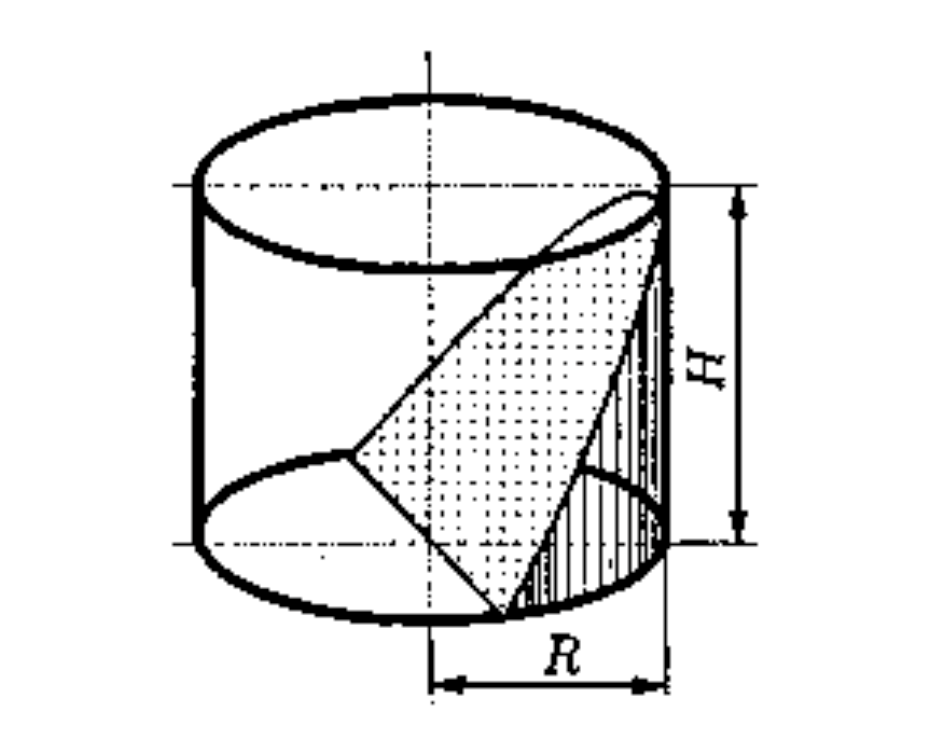
\includegraphics[scale=0.3]{pictures/cyltairdas.png}
        \item $h$ өндөртэй, $r$ ба $R$ суурийн радиустай огтлогдсон конусын эзэлхүүн бодох томьёог эргэлтийн биеийн эзэлхүүн олох томьёог ашиглан гарга. $r=R=2$ үед бодож шалга.
    \end{enumerate}
\end{enumerate}